\epigraph{\textit{We cannot solve problems with the kind of thinking we employed when we came up with them.}}{-- \textup{Albert Einstein}}

During the following paragraphs I am covering the motivation, contributions and structure of the document. This means, after reading it, you are building the big picture; a general idea of the motivations to develop this project, the results we are looking for and the shape of the it.

\section{Motivation}

These days, more and more devices are connected among them. Not only that, but tons of information is being stored automatically. This makes the task of having to process that data a complexer job. What's more, it is also becoming a more relevant assignment. Simply stated, the amount of data outruns our capacity to consume it.

A solution to that is Big data: an emerging field on Software development where we process strong volumes of diverse information at a speed. Big data applications not only have to scan large amounts of inputs the faster they can, but the variety of sources that information comes from, makes interoperability a key concept we must deal with.

Knowledge graphs~\cite{https://doi.org/10.48550/arxiv.2110.11709} were popularized back in 2012 by Google~\cite{web:knowledge_graphs:google} as a tool to represent real world data reflecting relationships between entities in order to understand those links better. It happens that after Google's introduction, others embraced this approach: ranging from proprietary to open databases. Companies like Facebook, LinkedIn and Amazon are already using knowledge graphs~\cite{web:knowledge_graphs:use} in order to have a better understanding of their customers. Even though there exist several models associated with this technology, we are focusing on wikibase graphs.

Summing up, this project focuses on the analysis and implementation of a system to validate wikibase graphs -- an specific flavour of the so called knowledge graphs -- using big data techniques. To put that into perspective, as of October 1 2022, a compressed \gls{dumps} of Wikidata's database has a size of 109.04Gb~\cite{wikidata:dumps}. Not only that, but the size of these dumps have exponentially increased with each and every release of a new one (see figure \ref{fig:dumps}).

\begin{figure}[h]
    \centering
    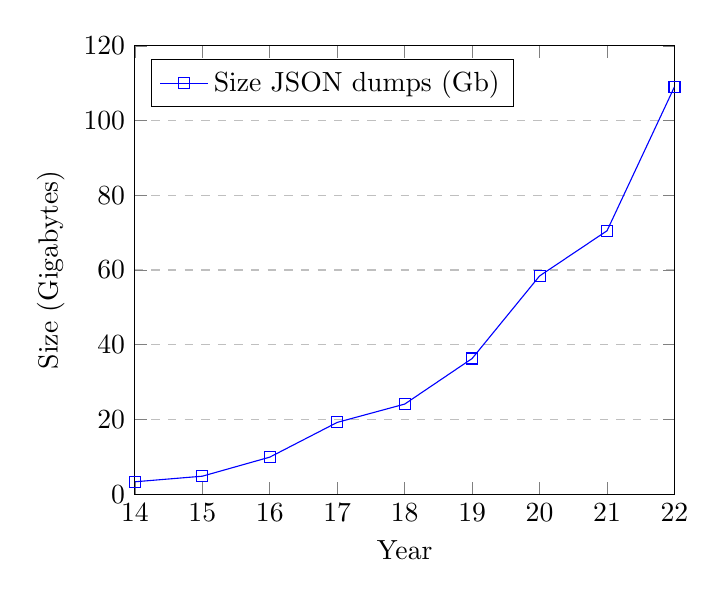
\begin{tikzpicture}
        \begin{axis}[
                title={},
                xlabel={Year},
                ylabel={Size (Gigabytes)},
                xmin=14, xmax=22,
                ymin=0, ymax=120,
                xtick={14,15,16,17,18,19,20,21,22},
                ytick={0,20,40,60,80,100,120},
                legend pos=north west,
                ymajorgrids=true,
                grid style=dashed,
            ]

            \addplot[
                color=blue,
                mark=square,
            ]
            coordinates {
                    (14,3.3)(15,4.8)(16,9.9)(17,19.2)(18,24.1)(19,36.3)(20,58.4)(21,70.5)(22,109.04)
                };
            \legend{Size JSON dumps (Gb)}
        \end{axis}
    \end{tikzpicture}
    \caption{Size of compressed wikidata dumps between 2014-2022~\cite{web:wikidata:dumps}}
    \label{fig:dumps}
\end{figure}

\textbf{Project's Goal 1.} \textit{Design and implementation of a system allowing us to validate huge dumps from Wikidata generating a subset out of it.} As we have in these introductory lines, the task of having to process enormous amounts of data is becoming increasingly relevant. A system that allows us to accomplish it the faster, the better solution we will provide.

\textbf{Project's Goal 2.} \textit{Reproduce an experiment related to the analysis of the previously described algorithm.} In order for us to properly analyze the results emerging from the execution of the algorithm we have implemented, we have to create a ecosystem were we can obtain information related to memory consumption, execution time, to name a few.

\textbf{Project's Goal 3.} \textit{Learn new technologies and Big data techniques.}

\section{Contributions}

The main contributions of this project are:

\begin{enumerate}
    \item
\end{enumerate}

\section{Structure of the document}

The shape of this document is as follows:

\begin{itemize}
    \item \textbf{Chapter ~\ref{chapter:description}.} General description of the existing technologies related to knowledge graph validation. As well as other tools related to this project.
    \item \textbf{Chapter ~\ref{chapter:theory}.} Provides a theoretical background needed for understanding the concepts explained in the following chapters.
    \item \textbf{Chapter ~\ref{chapter:experiment}.} Explanation of the process followed to analyze the concrete implementation of the algorithm that I used to validate the knowledge graphs.
    \item \textbf{Chapter ~\ref{chapter:results}.} Analysis of the results obtained from the previously described experiment.
    \item \textbf{Chapter ~\ref{chapter:conclusions}.} Summary of the general conclusions and future work.
\end{itemize}